\chapter{Zásuvný modul}
\label{4-plugin}

Ve této kapitole jsou objasněny stěžejní kroky tvorby zásuvného modulu
\textit{Radiation reconnaissance results}, popsány vstupní a výstupní
datové soubory. Při tvorbě modulu byly využívány příručky \cite{diveintopython} 
\cite{cookbook} \cite{qgis} \cite{ucebnicepython}.
%%% ML: vetu dokoncit...

\section{Vstupní data}

Na vstupu zásuvného modulu je buď interpolovaná mapa dávkového
příkonu, nebo plošné aktivity.

\begin{itemize}
\item \textbf{Interpolovaná mapa plošné aktivity}

  Mapa obsahuje hodnoty plošné aktivity v jednotkách
  {[}MBq/m$^2${]}. Je v souřadnicovém systému \zk{WGS 84} (EPGS:4326)
  a v gridovém formátu podporovaném knihovnou GDAL.

\item \textbf{Interpolovaná mapa dávkového příkonu}

  Mapa obsahuje hodnoty dávkového příkonu v jednotkách cGy/h. Je v
  souřadnicovém systému \zk{WGS 84} (EPGS:4326) a v gridovém formátu
  podporovaném knihovnou
  GDAL\footnote{\url{http://www.gdal.org/frmt_various.html}}.
	
\end{itemize}

\subsection{Testovací data}

\begin{figure}[H]
    \centering
      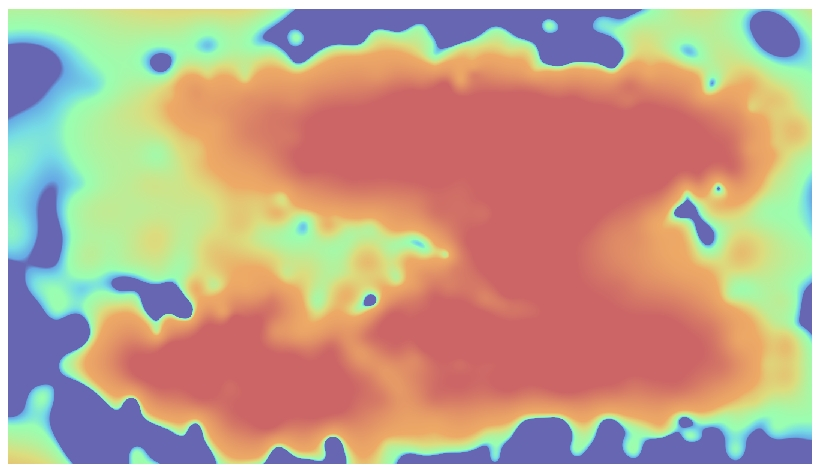
\includegraphics[width=300pt]{./pictures/chagan_spline.jpg}
      \caption[Interpolovaná mapa]{Interpolovaná mapa dávkového příkonu (Chagan Lake) (autor: Tereza Kulovaná, data: \zk{AČR})}
      \label{fig:spline}
\end{figure}

Bodová data pro testování poskytla \zk{AČR}. Jedná se o hodnoty
simulované pro účely cvičení umístěné do oblasti jezera Chagan
(přezdívaného "Atomic lake") v~Kazachstánu. Toto jezero vzniklo v roce
1965 jako důsledek sovětského podzemního jader\-ného testu (ekvivalentní
140 kt TNT) \cite{Nordyke2000}.

Atributová tabulka bodových dat obsahuje informace o měřených
hodnotách dávkového příkonu a plošné aktivity, souřadnicích X a
Y. Interpolovaná mapa dávko\-vého příkonu, resp. plošné aktivity, byla
vytvořena pomocí metody Multilevel B-Spline Interpolation v open
source \zk{GIS} softwaru
SAGA\footnote{\url{http://www.saga-gis.org/saga_tool_doc/2.1.3/grid_spline_4.html}}.
  
\begin{figure}[H] \centering
      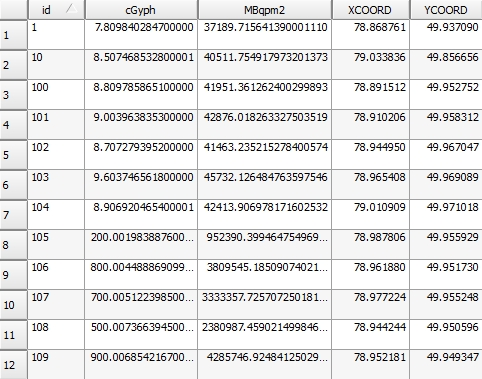
\includegraphics[width=270pt]{./pictures/chagan_attr.jpg}
      \caption[Atributová tabulka bodových dat (Chagan
      Lake)]{Atributová tabulka bodových dat (Chagan Lake) (autor:
        Tereza Kulovaná, data: \zk{AČR})}
      \label{fig:attributes}
\end{figure}

\section{Výstupní data}
\label{output}

\begin{enumerate}
	\item \textbf{Report}

          Povinným výstupem zásuvného modulu je textový report s
          příponou \textit{.txt}, který obsahuje souřadnice lomových
          bodů zjednodušených polygonů v hlásném systému
          \zk{MGRS}. Výstupní report je součástí \zk{MTF} zprávy,
          proto musí splňovat přesně daný formát specifikovaný v
          katalogu APP-11.

\newpage
Jeden řádek reportu obsahuje:

/[VALUE][UNIT]/MGRS:[COORDINATE]/MGRS:[COORDINATE]//

kde
\begin{itemize}
			\item VALUE = hodnota dávkového příkonu/plošné aktivity 
			
			\item UNIT = použitá jednotka ve formátu:
			
			\begin{itemize}
				\item v případě dávkového příkonu: XYH, kde
			 		\begin{itemize}
						\item X = C (\textit{centi}), M (\textit{mili}), U (\textit{mikro})
						\item Y = G (\textit{gray})
						\item H = H (\textit{hodina})
					\end{itemize}
				\item v případě plošné aktivity: BQM2 (\textit{becquerel na čtvereční metr})
			\end{itemize}
			
			\item COORDINATE = souřadnice v systému \zk{MGRS}
\end{itemize}
				
U hodnoty VALUE je oddělovačem desetinných míst desetinná
tečka. Veškerý text musí být velkými písmeny. Report musí začínat
lomítkem, vše mezi dvěma lomítky je nazýváno polem. Pole č. 1 může
obsahovat maximálně 12 znaků. Pole č. 2 může mít až 50 opakování
(maximum 50 souřadnic) a každé pole může za identifikátorem MGRS:
obsahovat maximálně 15 znaků. Poslední souřadnice je zakončena
dvojitým lomítkem (označuje konec řádku). Vše mezi prvním lomítkem a
dvojitým ukončovacím lomítkem se nazývá řádek. Jednotlivé řádky musí
%%% ML: enterem -> zalomeni radky (btw. pouziva se Unixovy nebo Windows zapis?)
%%% TK: používám os.linesep, mám to nahradit \n?
být odděleny znakem zalomení řádky.

\begin{figure}[H]
    \centering
      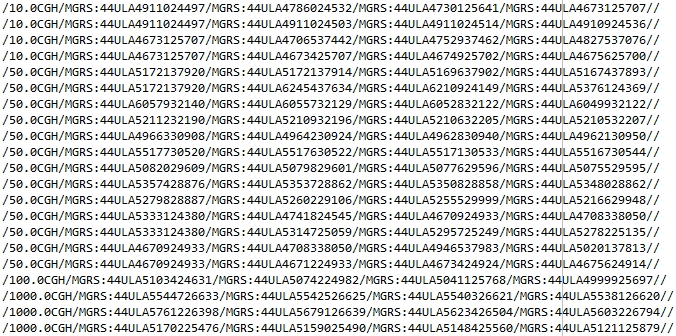
\includegraphics[width=375pt]{./pictures/vystupni_report.jpg}
      \caption[Výstupní report]{Ukázka výstupního reportu (autor: Tereza Kulovaná)}
      \label{fig:report}
\end{figure}

QGIS nemá nativní podporu souřadnic v \zk{MGRS}. Pro převod z~\zk{WGS
  84} do~\zk{MGRS} byla jako nejvhodnější z dostupných variant zvolena
část kódu již existujícího zásuvného modulu \textit{Lat Lon Tools
  Plugin}\footnote{\url{https://github.com/NationalSecurityAgency/qgis-latlontools-plugin}}. Konkrétně
se jedná o soubor s názvem \texttt{mgrs.py} a v něm obsaženou metodu
\texttt{toMgrs}. Tento zásuvný modul je distribuován pod licencí GNU
\zk{GPL}, stejnou jako vytvářený modul \textit{Radiation
  reconnaissance results}, což umožnilo jeho využití.

	\item \textbf{Soubor polygonů}
	
          Volitelným výstupem zásuvného modulu je datový soubor s
          polygonovými prvky. Data jsou lokalizována v souřadnicovém
          systému \zk{WGS 84} (EPGS:4326) ve formátu Esri Shapefile
          (\textit{.shp}). Datový soubor obsahuje geometrie
          zjednodušených polygonů různě graficky odlišené podle
          jednotlivých úrovní radiace. Atributová tabulka obsahuje:

		\begin{itemize}
			\item{identifikační číslo polygonu}
			\item{úroveň radiace}
		\end{itemize}

%%% ML: symbolizovat podle nejake vhodne skaly?
%%% TK: přidán barevnější obrázek
\begin{figure}[H]
    \centering
      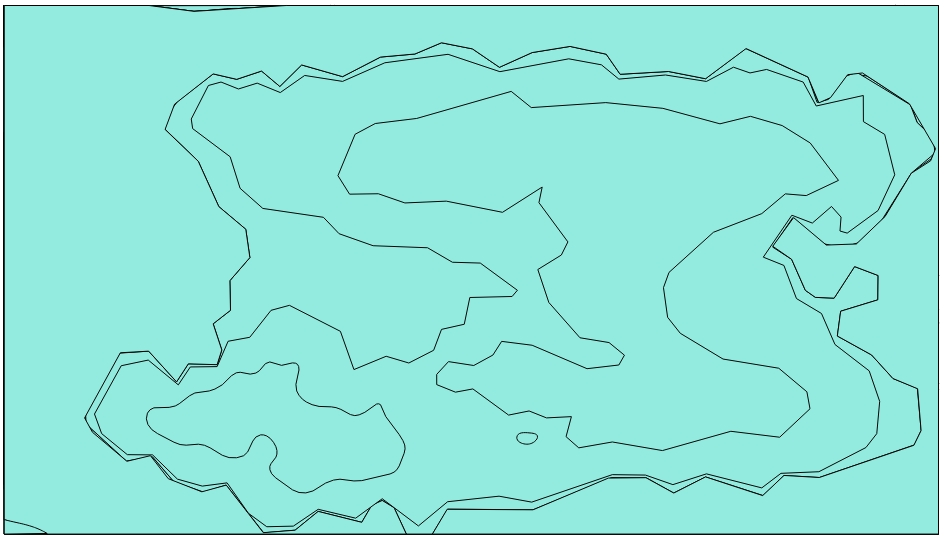
\includegraphics[width=300pt]{./pictures/vystupni_polygony.jpg}
      \caption[Výstupní polygony]{Ukázka výstupního souboru polygonů (autor: Tereza Kulovaná)}
      \label{fig:polygony}
\end{figure}

% obrázek bude upraven (z důvodu správného rozložení stránek)

\end{enumerate}

\section{Tělo zásuvného modulu}

Základní šablona nově vyvíjeného zásuvného modulu byla vytvořena s
pomocí volně dostupného zásuvného modulu \textit{Plugin
  Builder}\footnote{\url{https://plugins.qgis.org/plugins/pluginbuilder/}}. Autorem
tohoto modulu je skupina GeoApt LLC specializující se na rozvoj open
source softwaru. Po zadání povinných vstupních informací
\textit{Plugin Builder} vyprodukuje kostru zásuvného modulu tvořenou
mj. prvotním grafickým uživatelským rozhraním, základními funkcemi,
vazbami a~vychozí ikonkou.

Tuto základní kostru bylo třeba upravit a rozšířit o další soubory,
aby bylo docíleno očekávané funkčnosti. Mezi nejdůležitější prvky
zásuvného modulu patří několik navzájem provázaných souborů:

\begin{itemize}
	\item \textbf{\_\_init\_\_.py} 
	
	Obsahuje základní inicializaci modulu.
		
	\item \textbf{plugin\_upload.py} 

          Umožňuje nahrání modulu do repozitáře QGIS, odkud je
          dostupný komukoli.

	\item \textbf{radiation\_reconnaissance\_results.py} 
	
          Zajišťuje implementaci zásuvného modulu do prostředí QGIS -
          načtení ikonky s~názvem do nástrojové lišty, aktivaci modulu
          a v případě zavření jeho destrukci.

	\item \textbf{radiation\_reconnaissance\_results\_dockwidget.py}
	
          Obstarává propojení se souborem\\
          \textbf{radiation\_reconnaissance\_results\_dockwidget\_base.ui},
          po jehož zavolání se zobrazí grafické uživatelské rozhraní
          vytvořené pomocí Qt Designer. Obsahuje třídu
          \texttt{RadiationReconnaissanceResultsDockWidget} s metodami
          zajišťujícími načtení vstupních dat, předání potřebných
          hodnot dalším výpočetním souborům a v případě volby
          uživatele i přidání výsledné vrstvy polygonů do mapového
          okna. Dále znemožňuje spuštění modulu v situaci, kdy není
          zadána cesta k výstupnímu reportu.

	\item \textbf{pyradiation}

          %%% ML: Zminit, ze jde o knihovnu, ktera neni zavisla na
          %%% QGIS pluginu a muze byt pouzivata mimo nej, to je
          %%% dulezite
          Adresář \textbf{pyradiation} obsahuje knihovnu několika 
          vzájemně provázaných modulů zajišťujících výpočty a tvorbu
          %%% ML: spise nez o souboru muzete mluvit o "modulu" Jinak
          %%% na tomto miste zminte hlavne dane tridy
          výstupů. Tato knihovna čerpá pouze z knihovny \zk{GDAL} a 
          lze ji využít nezávisle na QGIS modulu.

          Ve třídě \texttt{RadiationIsolines} jsou ze vstupního
          gridu vytvořeny izolinie v uživatelem zvolených úrovních
          radiace. Datový soubor s~izoliniemi je předán dále třídě
          \texttt{RadiationPolygonizer}, kde jsou z nich vytvořeny
          zjednodušené polygony pomocí generalizace obsažené v modulu
          \texttt{generalizer.py} a k němu náležející třídě
          \texttt{RadiationGeneralizer}. Na závěr jsou ve třídě \texttt{RadiationReport}
          souřadnice lomových bodů polygonu převedeny do souřadnic
          systému \zk{MGRS} a v zadaném formátu vypsány do výstupního
          textového reportu.
	
\end{itemize}

\section{Algoritmus}

\begin{figure}[H]
    \centering
      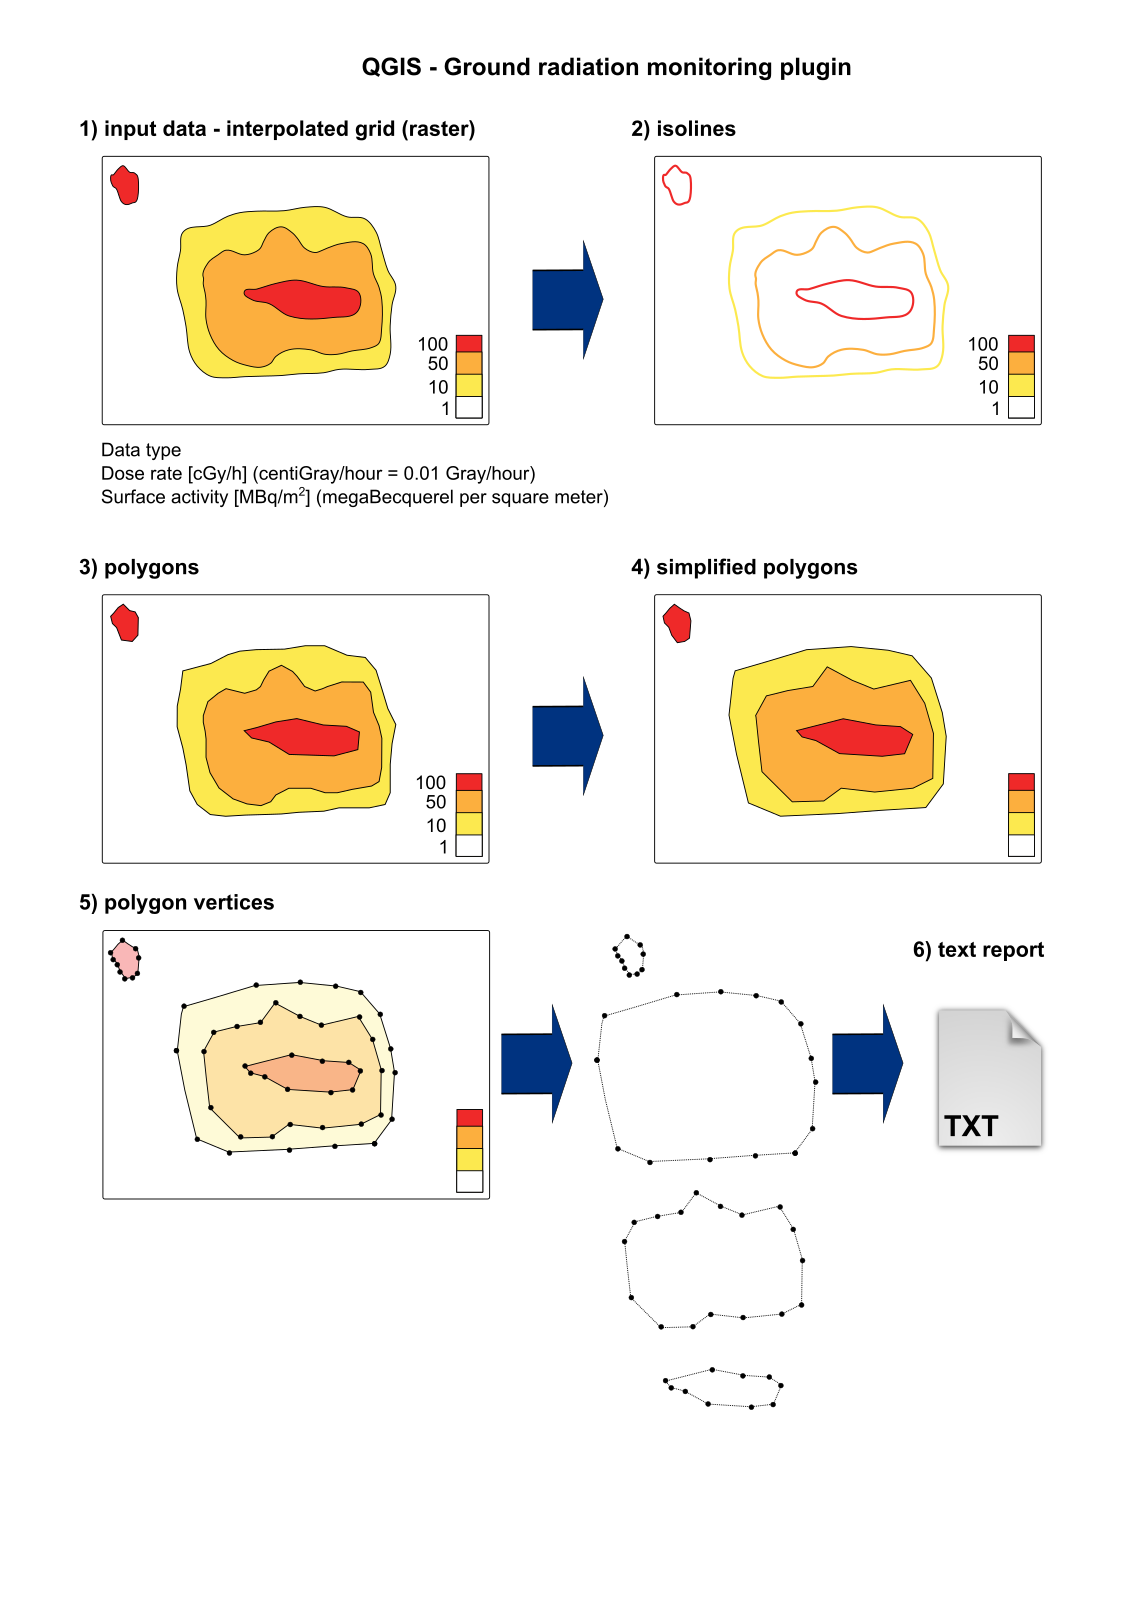
\includegraphics[width=300pt]{./pictures/ACR_radiacni_pruzkum_polygony_v3.png}
      \caption[Schematický postup]{Schematický postup (autor: \zk{SÚRO}, v.v.i.)}
      \label{fig:schema}
\end{figure}

V dalších kapitolách jsou představeny dílčí kroky postupu tvorby
koncových zjedno\-dušených polygonů.

\subsection{Tvorba izolinií}

V první fázi jsou ze vstupního gridu vytvořeny izolinie pomocí metody
\texttt{ContourGene\-rate} z~knihovny \zk{GDAL}. Vstupní grid ovšem
zahrnuje pouze ohraničené pole bez~informací z~okolí, což v~důsledku znamená, že
%%% ML: skutecnost -> okoli ?
část izolinií netvoří uzavřené oblasti, ale začíná a končí 
na~hranicích gridu a není uzavřena. Z těchto izolinií by nebylo možné
vytvořit polygony, které na~vstupu vyžadují uzavřenou oblast. Z~tohoto
důvodu je třeba tyto linie najít a uzavřít pomocí ohraničujícího
obdélníku.

V prvním kroku jsou určeny izolinie, které nejsou uzavřené
(pseudokód~\ref{alg:getIntersection}-4), a~pro~ně jsou vypočítány
průsečíky s ohraničujícím obdélníkem
(pseudokód~\ref{alg:getIntersection}-5). Tyto průsečíky linií jsou
přidány do pole průsečíků (pseudokód~\ref{alg:getIntersection}-9)
stejně jako rohové body ohraničujícího obdélníku
(pseudokód~\ref{alg:getIntersection}-14). Body v tomto poli jsou
seřazeny proti směru hodinových ručiček
(pseudokód~\ref{alg:getIntersection}-15). Při tvorbě izolinií metodou
\texttt{ContourGenerate} mohou vzniknout i linie, které nejsou
uzavřené a zároveň nekončí na hranicích obdélníka, ty je třeba z
vrstvy izolinií odstranit (pseudokód~\ref{alg:getIntersection}-7).

\begin{algorithm}
\caption{Získání průsečíků s ohraničujícím obdélníkem (Hranice)}
\label{alg:getIntersection}
    \begin{algorithmic}[1] 
    \STATE{vrstvaIzolinie = vrstva izolinií vypočítaných pomocí ContourGenerate}
    \STATE{izolinie = načti první izolinii z vrstvaIzolinie}
    \WHILE{existuje izolinie}
    	\IF{izolinie je neuzavřená}
    		\STATE{průsečík = vypočtiPrůsečíkyIzolinieAHranice}
    		\IF{neexistuje průsečík}		
				\STATE{odstraň izolinii z vrstvaIzolinie}
			\ELSE
				\STATE{přidej průsečík do polePrůsečíky}
			\ENDIF	
		\ENDIF
		\STATE{izolinie = načti další izolinii z vrstvaIzolinie}
	\ENDWHILE
	\STATE{přidej rohové body Hranice do polePrůsečíky}
	\STATE{seřaď polePrůsečíky proti směru hodinových ručiček}
    \end{algorithmic}
\end{algorithm}

V druhém kroku již dochází přímo k uzavírání linií. Základní postup je
přidat první izolinii do nově uzavírané linie
(pseudokód~\ref{alg:closeLines}-4). Pak jsou procházeny průsečíky na
obdélníku, dokud není nalezen další bod se stejnou úrovní radiace
(pseudokód~\ref{alg:closeLines}-9) a linie mezi ním a posledním bodem
je přidána do nově uzavírané linie
(pseudokód~\ref{alg:closeLines}-10). Pokud se jedná o počáteční bod
první izolinie, je linie uzavřená
(pseudokód~\ref{alg:closeLines}-11). Pokud se jedná o bod z jiné
izolinie, je tato izolinie přidána do uzavírané linie
(pseudokód~\ref{alg:closeLines}-24) a znovu se hledá další bod se
stejnou úrovní radiace. Tento postup se opakuje, dokud poslední
přidaný bod neodpovídá počátečnímu bodu první izolinie.


\begin{algorithm}
\caption{Uzavření linií}
\label{alg:closeLines}
    \begin{algorithmic}[1] 
    \STATE{neuzavřenéIzolinie = vrstva neuzavřených izolinií}
    \STATE{izolinie = načti první izolinii z neuzavřenéIzolinie}
    \WHILE{existuje izolinie}
    	\STATE{přidej izolinii do uzavíranáIzolinie}
    	\STATE{počátečníBod = počáteční bod izolinie}
    	\STATE{koncovýBod = koncový bod izolinie}
		\FOR{průsečík z polePrůsečíky}
    		\IF{průsečík po Hranici dál než koncovýBod}	
    			\IF{úroveňPrůsečík = úroveňIzolinie}								
					\STATE{přidej linii mezi koncovýBod a průsečík do uzavíranáIzolinie}
						\IF{průsečík = počátečníBod}
							\STATE{uzavíranáLinie je uzavřena -> \textbf{konec výpočtu}}
						\ELSE
							\STATE{koncovýBod = průsečík}
							\STATE{pokračuj na řádku 22}
						\ENDIF
%					\ELIF{úroveňPrůsečík = 0}
%						\STATE{rohHranice = průsečík}
%						\STATE{přidej linii mezi koncovýBod a rohHranice do uzavíranáIzolinie}
%						\STATE{koncovýBod = rohHranice}
%						\STATE{pokračuj s dalším průsečíkem}
				\ELSE
					\STATE{pokračuj s dalším průsečíkem}
				\ENDIF
			\ENDIF
		\ENDFOR
	\algstore{myalg}
	\end{algorithmic}
\end{algorithm}

\begin{algorithm}
	\begin{algorithmic} [1] \algrestore{myalg}
				\WHILE{uzavíranáLinie není uzavřená}
			\FOR{izolinie z neuzavřenéIzolinie}
				\IF{počátečníBodIzolinie = koncovýBod}
					\STATE{přidej izolinii do uzavíranáIzolinie}
					\STATE{koncovýBod = koncovýBodIzolinie}
					\STATE{pokračuj na řádce 7}
				\ENDIF
			\ENDFOR
		\ENDWHILE
		\STATE{izolinie = načti další izolinii z vrstvaIzolinie}
	\ENDWHILE
    \end{algorithmic}
\end{algorithm}

\newpage
\subsection{Tvorba polygonů}

Z uzavřených izolinií jsou pomocí metody
\texttt{BuildPolygonFromEdges} z knihovny OGR vytvořeny
polygony. Následně jsou zjednodušeny s využitím metody
\texttt{Simplify} ze stejné knihovny. Nakonec jsou souřadnice
zjednodušených polygonů převedeny do systému \zk{MGRS} a vypsány do
textového reportu kompatibilního s formátem dle
APP-11\footnote{\url{https://nhqc3s.hq.nato.int/Apps/Architecture/NISP2/std.aspx?vndb=standards&sbbs=y&refid=nato-app-11-d}}.
%%% TK: Přímo katalog k dispozici nemám.

%%% ML: rozdelit do dvou stranek... (detail, klidne to tak nechate)
\begin{algorithm}
\caption{Tvorba a zjednodušení polygonů}
\label{alg:polygon}
    \begin{algorithmic}[1] 
    \STATE{uzavřenéIzolinie = vrstva uzavřených izolinií}
    \STATE{izolinie = načti první izolinii z uzavřenéIzolinie}
    \WHILE{existuje izolinie}
		\STATE{vytvoř polygon metodou \texttt{BuildPolygonFromEdges}}
		\STATE{tolerance = prvotní volba tolerance}
		\WHILE{True}
			\STATE{zjednoduš polygon metodou \texttt{Simplify} s danou tolerancí}
			\IF{počet bodů v polygonu < 50}
				\STATE{konec}
			\ELSE
				\STATE{tolerance = větší tolerance}
			\ENDIF
		\ENDWHILE	
		\STATE{izolinie = načti další izolinii z vrstvaIzolinie}
	\ENDWHILE
    \end{algorithmic}
\end{algorithm}

%%% ML: po rozdeleni nebude nova stranka treba
\newpage
\subsubsection{Generalizace}
Metoda \texttt{Simplify} z knihovny \zk{GDAL} využívá ke zjednodušení
linie algoritmus Douglas–Peucker (pseudokód~\ref{alg:RDP}). Tento
algoritmus patří k nejčastěji používaným generalizačním algoritmům v
oblasti \zk{GIS}. Na rozdíl od většiny generalizačních algoritmů
neodstraňuje z původní linie body nesplňující geometrickou podmínku,
ale naopak vytváří novou linii tvořenou body, které podmínku splňují.
	
Jedná se o rekurzivní algoritmus, který při zjednodušení řetězce mezi
body \textit{A} a~\textit{B} vezme hranu \textit{AB}. Pokud
nejvzdálenější bod (\textit{C}) původní linie je maximálně 
ve~vzdálenosti rovnající toleranci \textit{T}, pak je aproximace hrany
dostatečná. V opačném případě rozdělí hranu \textit{AB} v daném bodě
\textit{C}, čímž vzniknou hrany \textit{AC} a \textit{CB}. Ty jsou pak
rekurzivně aproximovány stejným
postupem. \cite{hershberger1992speeding}

Tento algoritmus nezachovává vzájemnou polohu linií, je tedy nutné
ještě dalšími úpravami ošetřit, aby se zjednodušené polygony vzájemně
neprotínaly. Tyto úpravy jsou však velmi časově náročné a autorka je
před odevzdáním bakalářské práce nestihla implementovat. Pro správnou
funkčnost zásuvného modulu jsou však nutné a bude na nich pokračovat
po odevzdání.
	
%	Jedná se o rekurzivní algoritmus, který kolem hrany (spojnice
% dvou bodů z nové linie) hledá body z původní linie mimo koridor o
% zadané toleranci T. Pokud žádný takový nenajde, hrana zůstane
% stejná. Pokud nějaký bod mimo koridor existuje, najde ten, který od
% hrany leží nejdále a vloží ho nové linie. Tím se původní hrana
% rozdělí na dvě. Následně testuje stejnou podmínku na nově
% vytvořených kratších spojnicích.

%%% ML: tady opet text nevychazi dobre...
\begin{figure}[H]
    \centering
      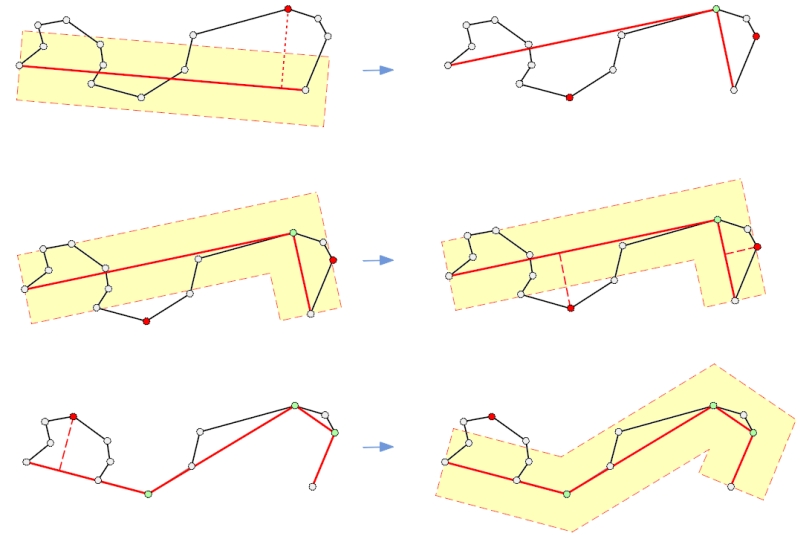
\includegraphics[width=350pt]{./pictures/DPalgoritmus.jpg}
      \caption[Ilustrace DP]{Ilustrace Douglas-Peucker algoritmu (zdroj: Ing. Tomáš Bayer, Ph.D., Přírodovědecká fakulta UK)}
      \label{fig:DPalgo}
\end{figure}	
	
\begin{algorithm}
\caption{Douglas–Peuckerův algoritmus}
\label{alg:RDP}
    \begin{algorithmic}[1] 
    \STATE{\textbf{funkce} DouglasPeucker(listBodů[], tolerance)}
    \STATE{dMax = 0}
    \STATE{index = 0}
    \STATE{početBodů = délka(listBodů)}
    \FOR{i = řada od 2 do (početBodů - 1)}
		\STATE{d = vzdálenost(listBodů[i], hrana(listBodů[1], listBodů[početBodů]))}
		\IF{d > dMax}
			\STATE{index = i}
			\STATE{dMax = d}
		\ENDIF	
	\ENDFOR
	\end{algorithmic}
\end{algorithm}	

\begin{algorithm}
    \begin{algorithmic}[1] 
	\IF{dMax > tolerance}
		\STATE{rekurze1 = DouglasPeucker(listBodů[1...index], tolerance)}
		\STATE{rekurze2 = DouglasPeucker(listBodů[index...početBodů], tolerance)}
		\STATE{výslednýList = {rekurze1[1...délka(rekurze1)-1], rekurze2[1...délka(rekurze2)]}}
	\ELSE
		\STATE{výslednýList = {listBodů[1], listBodů[početBodů]}}
	\ENDIF
	\STATE{\textbf{return} výslednýList[]}
    \end{algorithmic}
\end{algorithm}	

%%% ML: umele pouzit newpage (chtelo by text na poslednich 3-5
%%% strankach vice sladit (az bude finalni)
%%% TK: nakonec jsem zvolila přesun textu výše a rozdělení kódu
%%% do dvou částí, lepší verzi se mi vytvořit nepodařilo
\newpage

Zjednodušené polygony jsou předány třídě \texttt{RadiationReport} a 
je z~nich vytvořen výstupní textový report, jehož popis je uveden 
v~kapitole \ref{output}.

Návod k instalaci a použití zásuvného modulu je dostupný v přílohách (příloha \ref{user-guide}).